\documentclass[a4paper,11pt]{report}

\usepackage{alma}



\makeindex

\begin{document}


\begin{titlepage}

\vspace*{2cm}



\begin{flushleft}
	\hspace{1cm} \includegraphics*[width=4cm]{images/logo.jpg}\\
	\hspace{1cm} \textsl{Université de Nantes}\\
	\hspace{1cm} \textsl{12, rue de la Houssinière}\\
	\hspace{1cm} \textit{44322 Nantes}
	\hrulefill
\end{flushleft}




\vspace{2cm}

\begin{flushright}

	{\fontfamily{ppl}\fontseries{b}\fontsize{1.4cm}{1.65cm}\selectfont 
Alma Speech Recognition} 	 \\
	{\fontfamily{ppl}\fontseries{b}\fontsize{0.7cm}{0.825cm}\selectfont 
Projet de fin d'études} 	 \\

	
	\vspace{1cm}
	

	
	\vspace{1cm}
	Jérémy \textsc{Braud} \\
	Gaëtan \textsc{Hervouet} \\
	Cédric \textsc{Krommenhoek} \\
	Damien \textsc{Lévin} \\
	\textit{2009-2010}
	
\end{flushright}


\vspace{2cm}

\begin{flushleft}



	\hspace{1cm} \textsc{Master 2 - ALMA}\\
	
\end{flushleft}

\hspace*{0,5cm}\hrulefill
\end{titlepage}
% \hspace{\stretch{1}}


\begin{abstract}
Le projet de fin d'études consiste en la mise en \oe{}uvre de compétences acquises au cours des deux années de Master.
Chaque groupe de quatre à six étudiants travaille sur un sujet de projet différent.
Le déroulement du projet doit respecter les étapes de création d'un véritable projet open-source et doit en conséquent tirer au maximum profit des différents outils de gestion de projet.

Le projet que nous avons choisi de réaliser a été proposé par l'entreprise IBM~France\footnote{IBM~France -- \url{http://www.ibm.com/fr/fr/}}.
Il s'agit du fruit d'un partenariat entre IBM et l'Université de Nantes\footnote{La convention de partenariat a été signée le 24 novembre 2009.} afin de faciliter la scolarisation des étudiants malentendants.
En effet, à l'aide d'un logiciel disposant d'un moteur de reconnaissance vocale (en l'occurrence le moteur ``Speechroot'' d'IBM), l'étudiant aurait accès au sous-titrage du discours de l'enseignant de manière immédiate.
Ce projet diffère légèrement des autres par le fait que nous devons travailler en collaboration avec des groupes d'étudiants de d'autres écoles.
L'équipe d'IBM, composée de Béatrice~Martin et de sa collègue Christel~Amato, technicienne ayant une très importante expérience dans le domaine de la reconnaissance vocale, se charge de la coordination entre les trois groupes d'étudiants (celui de Centrale\footnote{Centrale Nantes -- \url{http://www.ec-nantes.fr/}}, de Polytech'\footnote{Polytech'Nantes -- \url{http://www.polytech.univ-nantes.fr/}} et nous-mêmes) et Stéphane~Brunat du Relai Handicap.
\end{abstract}

\tableofcontents


\chapter*{Introduction}
L'objectif de notre projet de fin d'études consiste à réaliser une application dans un temps imparti, en utilisant toutes nos compétences en matière de qualité logicielle et de gestion de projet.
Nous devons répondre aux exigences d'un client, M.~Brunat, pour que notre solution puisse être mise en place par l'Université.

Le choix des technologies à employer est libre, mais il nous faut im\-pé\-ra\-ti\-ve\-ment avoir quelque part dans notre architecture un code Java pouvant dialoguer avec le moteur Speechroot.
Ce moteur a été implémenté en C et nous n'avons pas l'autorisation de consulter ses sources, mais l'environnement JNI\footnote{Java Native Interface} permettant l'accès à ce code en java nous est fourni.


\chapter{Identification des besoins}

L'outil que nous développons est à destination d'étudiants malentendants.
Le profil de ces utilisateurs varie donc de l'utilisateur débutant à l'utilisateur avancé.
Pour être exploitable, notre logiciel doit donc être simple et fonctionnel à la fois. De plus, la prise en main doit être immédiate.

Pour des raisons évidentes, l'étudiant doit être en mesure de consulter la retranscription écrite du discours du professeur, et en même temps de rédiger des notes personnelles.
Ces données doivent être conservées de manière persistante afin de pouvoir les relire, les modifier ou les imprimer.
Pour que l'étudiant puisse travailler efficacement, les cours doivent être correctement triés selon des critères de classement par date de modification ou par module.

Pour que la reconnaissance vocale soit efficace, il faut absolument que le microphone employé soit de très haute qualité.
Le choix du microphone a été soumis à Mme Amato afin de profiter de son expérience dans ce domaine.
Il faudra tout de même effectuer quelques tests pour s'assurer que le microphone est bien adapté à l'usage que l'on souhaite en faire.

Dans l'idéal, nous aimerions que l'outil ne soit pas limité à certaines plateformes afin que l'étudiant puisse conserver la sienne.
Nous sommes conscients que le choix du moteur Speechroot va contraindre l'utilisateur à choisir Windows comme système d'exploitation, mais cette limitation peut toutefois être contournée par l'utilisation d'une machine virtuelle sur l'ordinateur de l'étudiant, à condition que celui-ci soit suffisamment performant.
Cette solution reste néanmoins complexe et n'est pas à la portée de n'importe quel utilisateur.
Il sera donc vivement conseillé aux étudiants novices en la matière de disposer de Windows.



\chapter{Architectures envisagés}

\section{Préambule}
Le cahier des charges présenté ci-dessus spécifie que l'application doit être
simple et mobile. Malgré certaines recommandations par le client, nous avons
tout de même étudié les choix qui s'offrait à nous en partant de l'existant.

\section{Système OrKestre}

Le système OrKestre est un système actuellement sur le marché. Il est aussi
connu sous le nom de système 'Perroquet'.

% 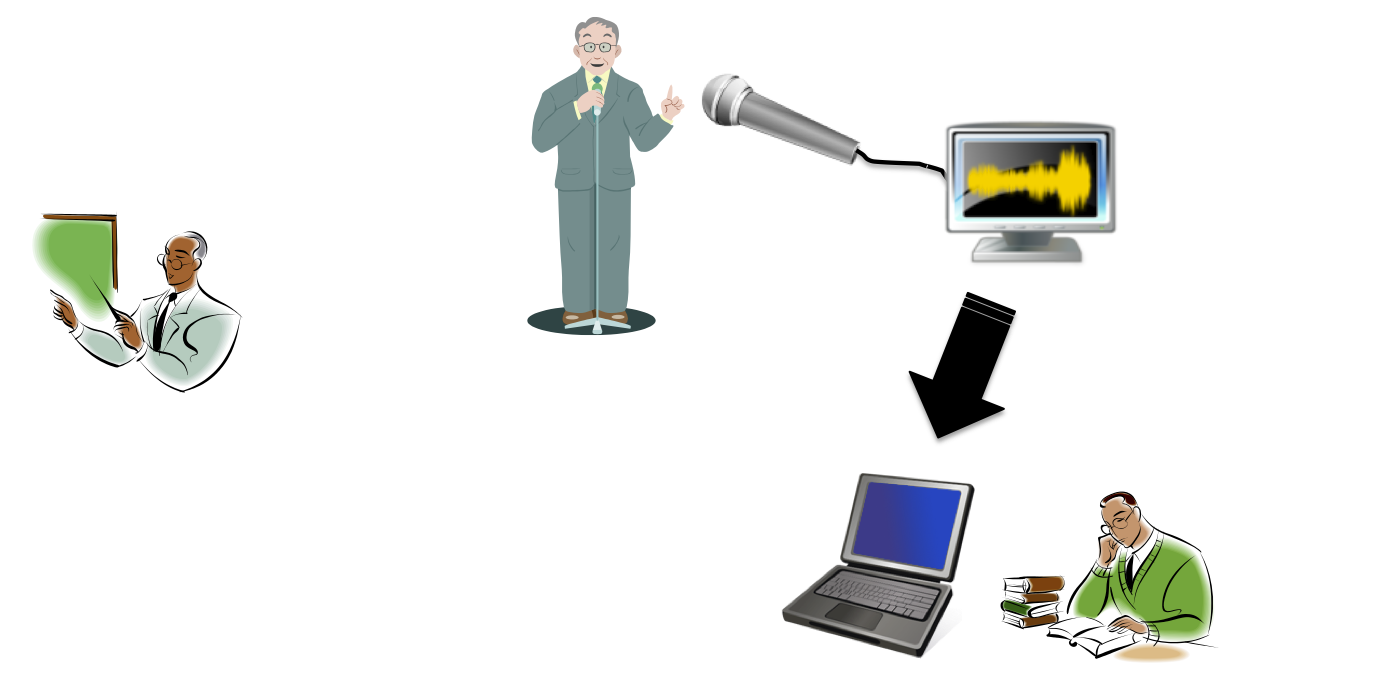
\includegraphics[width=12cm]{img/orKestre.png} 

Il se présente ainsi : Une personne est présente dans le cours et dicte distinctement le cours qu'elle entends du professeur, dans un microphone. Ce microphone est relié à un ordinateur qui dispose d'un moteur de reconnaissance vocale. Une fois le flux audio transformé en texte, ce dernier est envoyé à l'utilisateur malentendant par le réseau wifi ou filaire.

Ce système a pour avantage d'être optimal dans la qualité du texte reconnu par le moteur de reconnaissance vocale. En effet, le dicteur maitrise l'outil et y possède son dictionnaire ainsi que ses modèles vocaux. 
Pour autant, ce système n'est pas utilisable à l'université de Nantes car il nécessite l'engagement d'une personne tierce entièrement consacrée à la diction dans le microphone. Ceci est un problème pour l'université qui ne dispose pas de fond suffisant pour l'emploi et la formation d'une, voire de plusieurs personnes pour ce système.

\section{Solution 1}

% 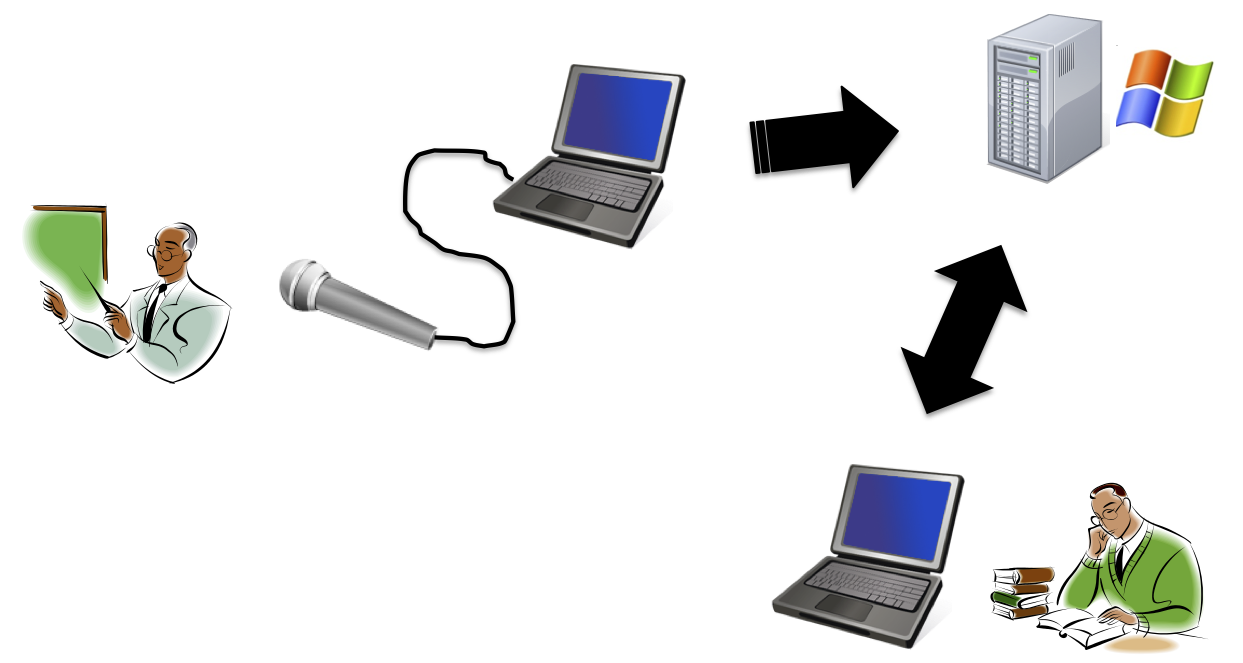
\includegraphics[width=12cm]{img/solution1.png} 

La première solution envisagée suit donc le modèle précédent mais sans une personne tierce.
Le microphone est donc directement relié à un ordinateur portable géré par le professeur.
Le son est transmit par cette ordinateur à un serveur fonctionnant sous Windows XP (requis pour faire tourner Speechroot) qui analyse le texte le transmet à un client web sur l'ordinateur de l'utilisateur malentendant.

\subsection{Pour}
Cette solution est la plus simple pour l'utilisateur. En effet, elle ne contraint pas celui-ci à utiliser un système d'exploitation tel que Windows Xp puisque le client web est compatible avec tout système qui fournit un navigateur web. Le texte serait donc affiché sur un site web interne à l'université.

\subsection{Contre}
Le problème est que cette solution n'est pas envisageable car certain professeurs sont ré\-frac\-tai\-res à l'informatique. Le professeur ne doit donc pas avoir à manipuler un ordinateur mais juste à porter le microphone.


\section{Solution 2}

La solution 2 reprends donc la solution précédente, mais on supprime l'ordinateur manipulé par le professeur.

%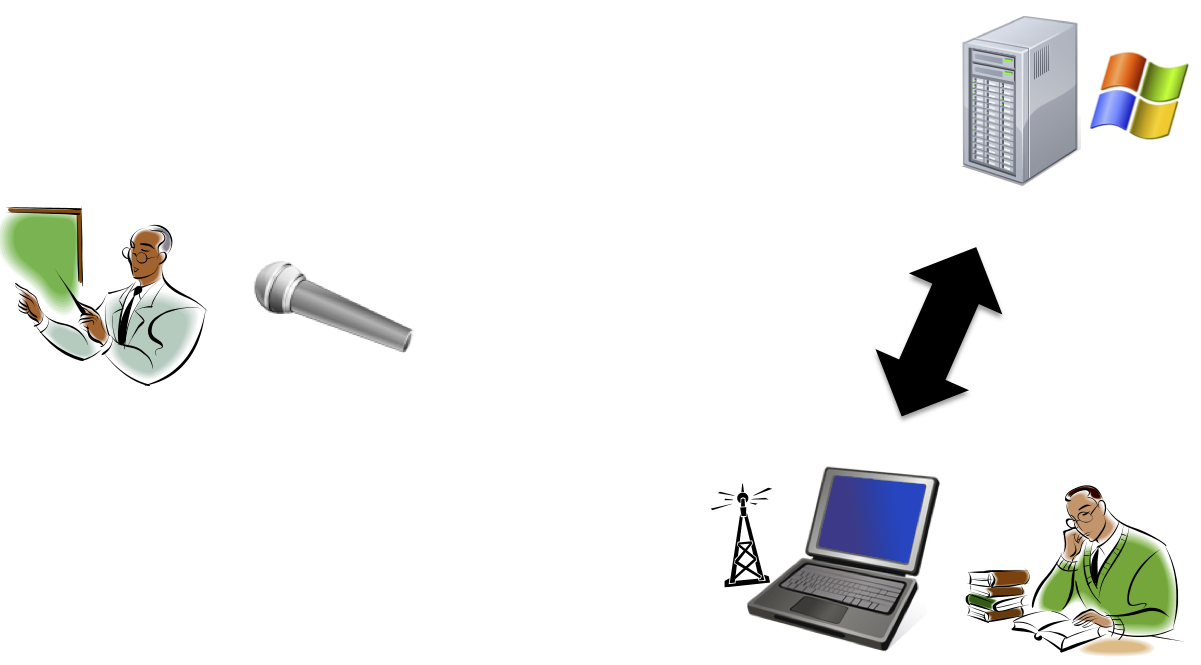
\includegraphics[width=12cm]{img/solution2.png} 

Le microphone perds son fil et est donc un récepteur est connecté à l'ordinateur de l'élève.
C'est donc par son ordinateur que le flux audio est transmis au serveur de l'université qui fait fonctionner le moteur de reconnaissance vocale.

Le texte lui est renvoyé, comme auparavant, dans un client web.

\subsection{pour}
Le professeur n'a pas à se soucier de l'ordinateur portable : l'élève connecte le micro du professeur à son ordinateur personnel.

\subsection{Contre}
Cette solution n'est tout de même pas envisageable à l'université. Bien qu'elle soit la plus simple et la plus mobile pour le professeur et l'elève, l'université refuse de maintenir un serveur fonctionnant sur Windows XP.

\section{Solution 3}
La solution 3 est finalement celle que nous avons choisi d'implémenter car c'est la seule qui est réalisable même si on perds en mobilité, utilisabilité et simplicité.

%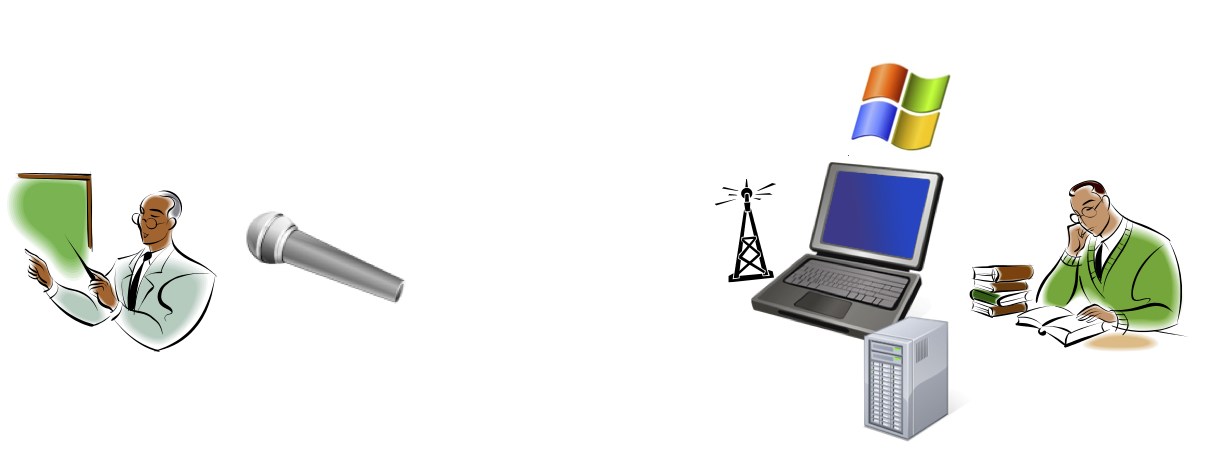
\includegraphics[width=12cm]{img/solution3.png} 

En effet, le moteur de reconnaissance vocale est finalement déplacé sur l'ordinateur personnel de l'étudiant : il est exécuté en tache de fond sur celui-ci. L'ordinateur de l'étudiant exécute donc un logiciel qui est uniquement compatible avec Windows. On perds donc en portabilité mais seule cette solution est réalisable.

\chapter{Développement de l'application}
\minitoc

\section{Intégration du moteur de reconnaissance vocale}

\subsection{Préambule}
La reconnaissance vocale de notre application s'effectue à l'aide du moteur Speechroot, développé il y a une dizaine d'années par l'entreprise IBM en langage C.
Pour des raisons de confidentialité, nous n'avons pas accès au code source de ce moteur mais à son interface nous permettant de l'exploiter.
Cette interface JNI va nous permettre d'intégrer le moteur dans notre application, écrite en Java.
Comme nous l'avons déjà signalé auparavant, ce moteur a été compilé pour Windows et ne peut donc pas être exécuté sur d'autres systèmes d'exploitation.

\subsection{Fonctionnalités du moteur}
A partir de l'interface JNI, nous avons accès à une liste de fonctionnalités que nous pouvons alors appeler.
Les fonctions de bases du moteur sont les suivantes~:
\begin{itemize}
\item démarrage et arrêt du moteur de reconnaissance vocale,
\item ouverture et fermeture du microphone,
\item ouverture de l'interface de gestion des dictionnaires,
\item ouverture de l'interface de gestion des modèles vocaux.
\end{itemize}	

Le moteur effectue ses retours à l'aide d'une fonction de callback que nous lui spécifions lors d'une initialisation obligatoire, avant son démarrage.
Cette fonction prend en paramètres deux chaînes de caractères représentant le type de message et son corps.
Les retours qui nous intéressent le plus sont donc ceux qui correspondent à résultat de la traduction effectuée par le moteur.
Ces retours sont identifiés par le type de message \texttt{onNewReco} et leur corps respecte la syntaxe~:
\begin{verbatim}
WORDS###confidence score###Pronunciation###begin word time//end word time
    ###flags
\end{verbatim}
où \texttt{WORDS} correspond aux mots reconnus et le reste aux paramètres du moteur.
Les paramètres correspondent à~:
\begin{description}
\item [\texttt{confidence score}~:] nombre compris entre -100 et 100 et qui représente au degré de confiance de la reconnaissance.
\item [\texttt{Pronunciation}~:] la prononciation des mots, similaire à l'alphabet phonétique international.
\item [\texttt{begin word time}~:] l'heure de début de la reconnaissance de ces mots.
\item [\texttt{end word time}~:] l'heure de fin de la reconnaissance de ces mots.
\item [\texttt{flags}~:] Drapeaux indiquant des informations supplémentaires telles que :
\begin{itemize}
\item le prochain mot commencera par une majuscule.
\item le prochain mot sera collé au précédent.
\item etc.
\end{itemize}
\end{description}

Le moteur offre également d'autres fonctionnalités que nous n'exploiterons pas, comme par exemple la reconnaissance vocale d'un fichier audio ou la possibilité de conserver le flux audio de la transcription.

\subsection{Intégration}
Afin que notre application soit évolutive au maximum et qu'elle ne dépende pas d'un unique moteur de reconnaissance vocale, nous avons conçu une interface disposant des fonctionnalités de base que nous avons énuméré auparavant (voir figure~\ref{fig:engineDiagram}).
Comme notre objectif est d'intégrer en particulier le moteur Speechroot, nous avons pensé cette interface de manière à ce qu'elle se calque parfaitement avec lui.

\begin{figure}[ht!]
 \centering
 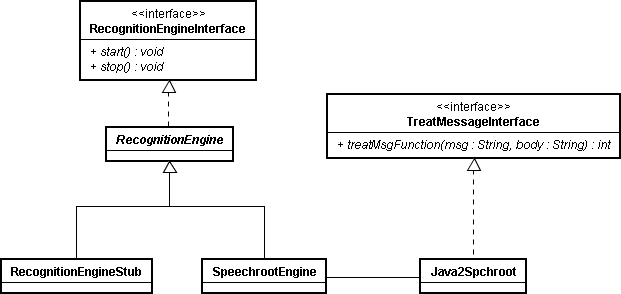
\includegraphics[scale=.5,keepaspectratio=true]{./images/EngineDiagram.png}
 % EngineDiagram.png: 621x294 pixel, 72dpi, 21.90x10.37 cm, bb=0 0 621 294
 \caption{Diagramme des classes du moteur de reconnaissance vocale}
 \label{fig:engineDiagram}
\end{figure}

La présence de la classe abstraite implémentant l'interface se justifie par le fait que le moteur est observé par le contrôleur de notre application.
Il doit en conséquent étendre la classe \texttt{java.util.Observable}, ce que nous ne pouvons pas spécifier avec seulement une interface.

Dans le cas de Speechroot, le moteur doit utiliser une classe implémentant l'interface fournie par IBM~: \texttt{TreatMessageInterface}.
Cette interface spécifie la fonction de callback qui doit être passée en paramètre lors du démarrage du moteur.
C'est donc dans l'implémentation de cette fonction que nous décodons le corps du message pour ensuite le transmettre au contrôleur à l'aide du patron de conception ``observateur''.

Nous avons rencontré quelques difficultés concernant les retours de callback du moteur Speechroot.
En effet, les retours ne s'effectuaient pas correctement~: nous ne les récupérions pas tant que nous n'exécutions pas un appel aux interfaces de gestion des dictionnaires ou des modèles vocaux.
Nous en avons déduis qu'il devait probablement y avoir un processus bloquant au sein du moteur.
Pour cette raison, nous avons écris rapidement un bouchon simulant l'action de ce moteur, afin de pouvoir poursuivre notre projet sans nous soucier de ce problème que nous ne pouvions pas régler seuls.
Puisque que tous ces moteurs étendent la même classe, et que c'est cette classe abstraite que nous appelons dans le contrôleur, il est extrêmement facile d'échanger le bouchon par le véritable moteur Speechroot, dès que le soucis de ce dernier sera réglé.
Bien que ce n'était pas notre intention originelle, nous avons préféré lors de notre soutenance faire la démonstration de notre application munie du bouchon plutôt que du moteur Speechroot pour montrer au mieux les possibilités qu'offrait notre interface graphique, cœur de notre projet.



\section{Déploiement de la base de données embarquée}

Afin de permettre l’enregistrement des cours de manière simple et intuitive, nous avons souhaité mettre en place une base de données. 
Cela permettra à l’utilisateur de classer les cours comme il le souhaite et de retrouver ces derniers rapidement, à la manière d’un client de messagerie.
Comme la base doit démarrer avec le programme, cette dernière doit être embarquée.
Nous avons choisi d’utiliser H2, base de données embarquée et légère, qui nous a été conseillée lors de notre formation.

Lors de la réalisation de cette base de données, nous avons utilisé surtout deux patrons de conception. 

Pour effectuer l’abstraction des données, l’utilisation du pattern DAO parait ici tout indiquée, cela permet de séparer les entités d'accès à la base de manière simple et fonctionnelle.
Il s'agit surtout de ne pas écrire ces accès dans les classes "métier", qui ne seront modifiées que si les règles de gestion métier changent.

Pour la conceptualisation de la base, nous avons utilisé le pattern composite.
Un objet composite est constitué d'un ou de plusieurs objets similaires (ayant des fonctionnalités similaires). 
L'idée est de manipuler un groupe d'objets de la même façon que s'il s'agissait d'un seul type d’objet, en utilisant leurs opérations communes.
Ici, nous avons voulu mettre en place des cours (fichiers) et des dossiers.
Nous en avons extrait les opérations communes et avons défini le type abstrait Element, qui devient alors classe mère des deux autres.
Une fois cela réalisé, le type dossier (Folder) peut alors référencer des éléments, sans se soucier du type final  (voir figure~\ref{fig:compositeDiagram}).

\begin{figure}[ht!]
 \centering
 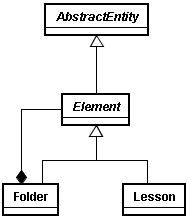
\includegraphics[scale=1,keepaspectratio=true]{./images/CompositeDiagram.png}
 \caption{Diagramme des classes de la base de données}
 \label{fig:compositeDiagram}
\end{figure}

Afin de gérer la persistance,  les classes « métiers » ont été annotées. Cela évite de faire un mappage XML pénible et potentiellement source d’erreurs.



\chapter{Interface homme machine}
\minitoc

\section{Fonctionnalités de l' IHM}

L'interface homme-machine est une des composantes essentielles de notre projet.
En effet, c'est en grande partie grâce à elle que l'utilisateur va pouvoir juger de la qualité du logiciel.
Ainsi, conformément au cahier des charges, on va retrouver les fonctionnalités suivantes~:

\begin{enumerate}

\item Editeur de texte~: Editeur conçu pour que l'utilisateur réalise des prises de notes.
L'éditeur est composé des éléments suivants~:
\begin{itemize}
\item Outils de formatage,
\item Affichage du plan.
\end{itemize}
\item Visualisation du cours~: Panneau pour visualiser le cours prononcé par l'enseignant, en provenance du moteur de reconnaissance vocale.
\item Explorateur de documents~: Possibilité pour l'utilisateur de parcourir ses cours et de les organiser.
On y retrouve les trois éléments suivants~:
\begin{itemize}
\item Module,
\item Dossier,
\item Cours.
\end{itemize}
\item Outils d'import et d'export~: Pour permettre à l'utilisateur d'utiliser ses supports de cours sur différentes plateformes ou encore de les imprimer, les fonctionnalités suivantes sont disponibles~:
\begin{itemize}
\item Export au format PDF,
\item Export/import au format RTF (Format Microsoft, compatible Word),
\item Impression du cours édité.
\end{itemize} 
\item Outils de configuration du moteur de reconnaissance vocale.  
\end{enumerate}

L'ensemble de ces fonctionnalités n'était pas figé lors du processus de développement, elles ont donc été ajoutées au fur et à mesure des cycles de celui-ci.

\section{Ergonomie}

\subsection{Solutions de visualisation et d'édition envisagées}

\subsubsection{Solution 1}

En ce qui concerne l'ergonomie du logiciel plusieurs choix de conception ont été mis en confrontation. Le premier, qui n'a finalement pas été retenu était d'utiliser un unique éditeur de texte. Celui-ci aurai joué un  double rôle, tout d'abord celui d'un panneau de visualisation du cours, prononcé par l'enseignant. Le cours aurai été affiché à la fin du document. De plus, l'utilisateur aurai eu la possibilité de modifier le panneau de visualisation dans le but d'organiser son  cours.

Le principal soucis de cette solution était que le travail de restructuration du cours en direct aurai été une tâche particulièrement fastidieuse et aurai fortement perturber la suivie du cours.


\subsubsection{Solution 2}

La solution finalement envisagée est l'utilisation de deux panneaux. Un premier dont le but est d'afficher le texte brut, issu du moteur de reconnaissance vocale. Celui-ci  va permettre à l'utilisateur malentendant d'utiliser sa  vision en remplacement de son ouïe. Le second panneau sert quand à lui de support de cours, offrant notamment la possibilité de prise de notes. De la même façon qu'un étudiant normal prendrai des notes sur papier.

Bien que cette solution semble la plus productive et la plus intéressante, elle est n'est pas exempt de défauts. Ainsi, il faut bien souligner le fait qu'il est particulièrement difficile de lire un texte tout en réalisant des prises de notes. Ainsi, même si cette solution semble plus difficile pour les utilisateurs moins familiers avec l'informatique, elle constitue pour nous la meilleure solution pour répondre au besoin de saisie d'un cours.On notera également que pour un utilisateur familier avec l'informatique, le fait de saisir un texte sans regarder le clavier ne pose pas de problèmes particuliers, lui laissant ainsi la possibilité de lire facilement le texte issue du moteur de reconnaissance.


\subsection{Accessibilité}

Un des points fondamentaux de l'IHM était de concevoir une interface intuitive et facile d'utilisation. Ainsi, un effort particulier à été consacré a l'accessibilité de l'outil, de sorte que l'utilisateur prenne rapidement en main l'outil. Pour cela, différents points ont étés réalisés :

\begin{enumerate}
 \item Une barre d'outils avec des icônes explicites : pour permettre un accès rapide au principales fonctions
 \item Création de raccourcis claviers classiques (CTRL-C, CTRL-V ...)
 \item Utilisation des standards d'ergonomie : Placement des menus, des boutons ...
\end{enumerate}

\subsection{Tests ergonomiques}

En raison de problèmes de temps, il n'a malheureusement pas été possible de réaliser des tests d'ergonomie avec un étudiant mal-entendant. Cependant  l'approche idéale pour la réalisation de cette IHM, aurai été de suive un cycle de développement basé sur des méthodes agiles orientées vers l'utilisateur. Notamment l'utilisation de XP, de Scrum ou encore de la méthode LUCID\footnote{devernay.free.fr/cours/IHM/lucid.pdf}.


\section{Conception MVC}

En ce qui concerne la conception de l'application elle s'organise suivant le pattern MVC\footnote{J2EE Architecture Approaches : http://java.sun.com/} : Model View Controler. Le but d'une telle architecture est de bien diviser les différentes couches de l'application. On retrouve ainsi une couche Model, gérant les entités de la base de donnée (utilisation du pattern DAO); une couche View, à laquelle on associe l'interface graphique réalisée en swing; et enfin une couche intermédiaire controller, qui comme son nom l'indique sert à contrôler les deux autres couches via des mécanismes de synchronisation, notamment via l'utilisation du pattern Observer. 



\begin{figure}[h]
 \centering
 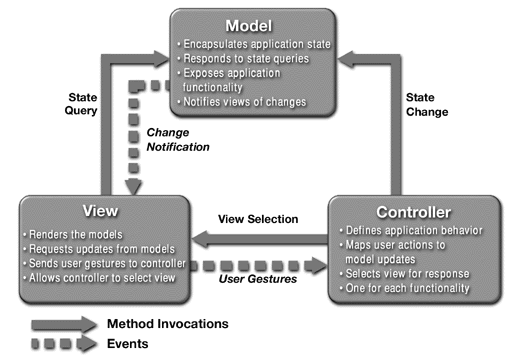
\includegraphics[scale=0.8]{./images/mvc.png}
 % homePanel.png: 0x0 pixel, -2147483648dpi, 0.00x0.00 cm, bb=
 \caption{IHM - Architecture MVC }
 \label{fig:mvc}
\end{figure}


Le diagramme \ref{fig:ihmUMLl} montre l'organisation des différentes classes de l'application. Comme on peut le voir, l'IHM est découpée suivant les principaux panels qui la compose. De plus, on distingue clairement la séparation entre les différentes couches de l'application. La classe Controller au centre, et le moteur de reconnaissance, qui ici fait office de couche Métier\footnote{Pour des raison de lisibilité, le module de gestion de la base de donnée n'est pas présent sur ce diagramme}.



\begin{figure}[h]
 \centering
 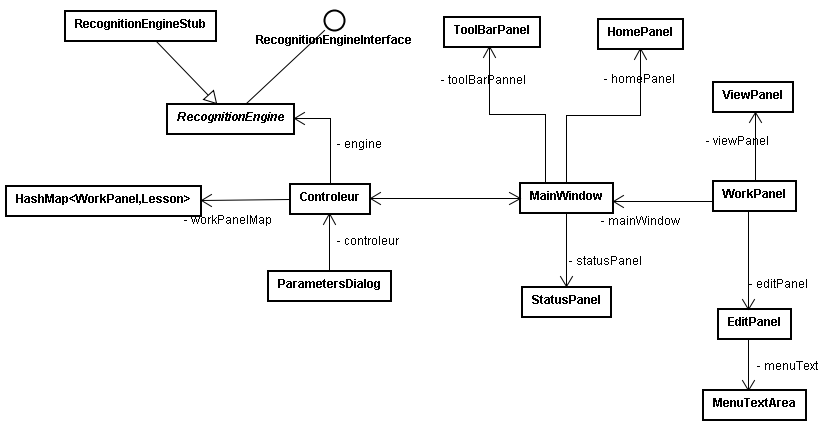
\includegraphics[scale=0.5]{./images/ihmUML.png}
 % homePanel.png: 0x0 pixel, -2147483648dpi, 0.00x0.00 cm, bb=
 \caption{IHM - Diagramme de classes}
 \label{fig:ihmUMLl}
\end{figure}


\section{Captures d'écran}

\subsection{Panneau d'accueil}


La figure \ref{fig:homePanel} montre le l'application au lancement de l'interface. Comme on peut le voir le panneau de gauche contient la liste des cours de l'utilisateur. Il peut ainsi les organiser facilement à la manière d'un explorateur de fichier classique. (Actions glisser déposer, création d'éléments ...). Sur la partie droite on retrouve la liste des documents de l'utilisateur. Cependant, pour des raisons d'ergonomie, ce panneau vise à offrir une organisation différente des cours. Il est ainsi possible de trier ses cours en fonction de leurs date de modification, de création ... Il faut noter que le changement de l'organisation sur ce panneau ne modifie pas l'organisation du panneau de gauche qui est indépendante.


\begin{figure}[H]
 \centering
 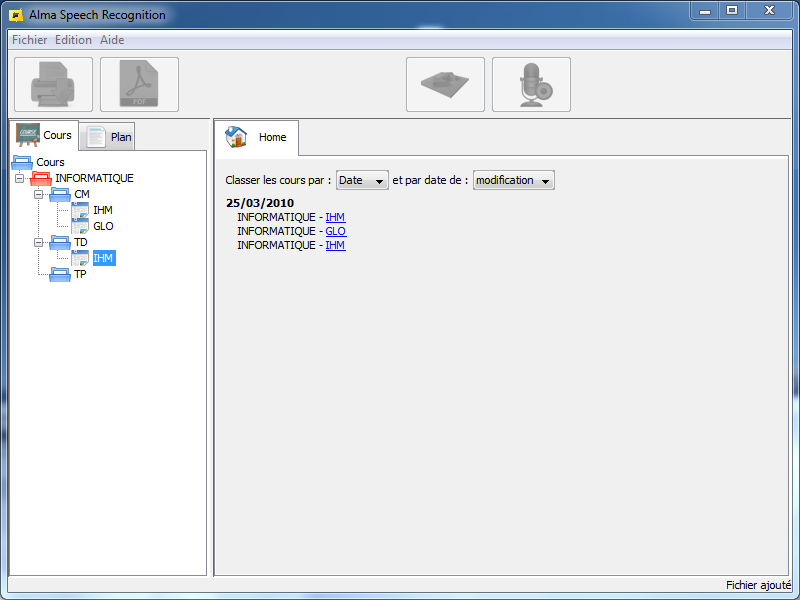
\includegraphics[scale=0.6]{./images/homePanel.png}
 % homePanel.png: 0x0 pixel, -2147483648dpi, 0.00x0.00 cm, bb=
 \caption{IHM - Panneau d'accueil}
 \label{fig:homePanel}
\end{figure}




\subsection{Panneau de travail}

La figure \ref{fig:workPanel} représente la même fenêtre que celle présente sur la figure \ref{fig:homePanel}. Cependant, ici on peut voir qu'un cours à été ouvert. L'ensemble des cours ouvert sont accessibles dans les différents onglets qui composent la fenêtre. Sur la figure \ref{fig:workPanel}, on remarque que les cours IMH et GLO sont ouverts simultanément.

Toujours sur cette fenêtre, on peut voir que chaque cours (onglet) se divise en deux parties : la partie visualisation du cours, qui affiche de façon continue la sortie du moteur de reconnaissance vocale, et la partie d'édition de texte, qui va servir de support de prises de notes pour l'utilisateur. 

Comme indiqué précédemment, l'aspect simplicité et rapidité d'utilisation est un élément fondamental dans cette IHM. Pour répondre à ce besoin, une barre d'outils à été conçue. Elle regroupe les actions principales pour manipuler le moteur de reconnaissance (Capture, Arrêt) mais également les fonctions annexes d'exportation de documents (PDF, impression). Un bouton pour stopper l'affichage continu du texte à également été ajouté. Il permet à l'utilisateur de se concentrer un instant sur un point particulier du texte, tout en ayant la possibilité de reprendre le fils du cours par la suite, sans perdre d'informations.



\begin{figure}[H]
 \centering
 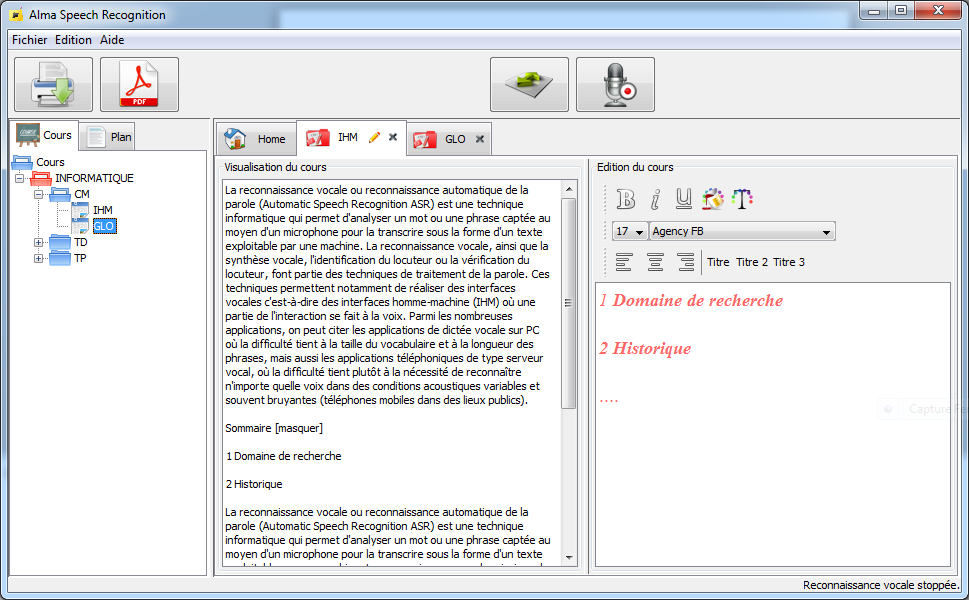
\includegraphics[scale=0.6]{./images/workPanel.png}
 % homePanel.png: 0x0 pixel, -2147483648dpi, 0.00x0.00 cm, bb=
 \caption{IHM - Panneau de travail}
 \label{fig:workPanel}
\end{figure}




\chapter{Qualité Logicielle}

Ce chapitre détaille les aspects de qualité logicielle qui ont été pris en compte tout le long du projet.

\section{Sonar}

60 révisions 
3640 lignes de codes 
Couverture de test de 100% sur la base de données
(IHM non testable) 
Respect des règles de style « checkstyle » (Convention syntaxique)
Utilisation de Sonar
 Evaluation du code 
 Détection des problèmes d’interdépendance 
 Calcul de la complexite


\chapter{Bilan}


\chapter{Conclusion}


\listoffigures   

\appendix

\chapter{Suivi de projet}

\begin{description}
\item[14 janvier~:] Premier contact avec l'équipe d'IBM, réunion de démarrage du projet au LINA\footnote{Laboratoire d'Informatique de Nantes-Atlantique} avec Mme~Martin, Mme~Amato et M.~Sunyé~; aperçu de la problématique et des besoins.
\item[19 janvier (matin)~:] Réunion hebdomadaire au LINA avec M.~Sunyé~; mise en place du dépôt Subversion.
\item[19 janvier (après-midi)~:] Premier contact avec M.~Brunat du Relai Handicap~; spécifications des besoins de l'utilisateur de l'outil, précisions sur les contraintes techniques.
\item[26 janvier~:] Réunion hebdomadaire~; discussion sur de nouveaux concepts à ajouter à l'outil.
\item[2 février~:] Réunion hebdomadaire~; répartition de tâches~: description des cas d'utilisation, spécification du schéma de la base de données embarquée, storyboard de l'IHM.
\item[9 février~:] Réunion au LINA avec l'équipe de Polytech'~; présentation des solutions architecturales envisageables, partage d'idées pour l'ergonomie de l'IHM.
\item[16 et 23 février~:] Réunions hebdomadaires~; discussion sur l'avancement du projet, engagement de démarche pour le choix du microphone.
\item[2 mars~:] Réunion hebdomadaire~; mise en place du système de gestion de projet Basecamp\footnote{Projet Basecamp -- \url{https://master-alma.basecamphq.com/}}
\item[9 mars~:] Réunion hebdomadaire~; découverte et exploitation du serveur d'intégration Hudson et du serveur de contrôle de qualité de code Sonar.
\item[11 mars~:] Conférence téléphonique au LINA avec M.~Sunyé, M.~Brunat et l'équipe d'IBM~; discussion sur l'avancement du projet et sur les difficultés rencontrées.
\item[16 mars~:] Dernière réunion hebdomadaire~; définition de nouvelles tâches à réaliser.
\item[25 mars~:] Soutenance du projet~; exposé et démonstration de l'outil.
\end{description}


\chapter{Diagramme de Gantt}

Bien que nous ne nous soyons pas vraiment attribués de fonctions telles que développeur, architecte ou même chef de projet, nous nous sommes répartis une grande partie des tâches à accomplir pour l'avancement du projet.
En conséquent, nous obtenons le diagramme de Gantt de la figure~\ref{}. %TODO


\printindex


\end{document}
